\section{Durchführung}
\label{sec:Durchfuehrung}



\subsection{Aufgaben}
\label{subsec:Aufgaben}

In Teil \textbf{a)} soll die Zeitkonstante des RC-Gliedes mit Hilfe der Schaltung in
Abbildung~\ref{fig:esb1} bestimmt werden.

\begin{figure}
    
    \centering
    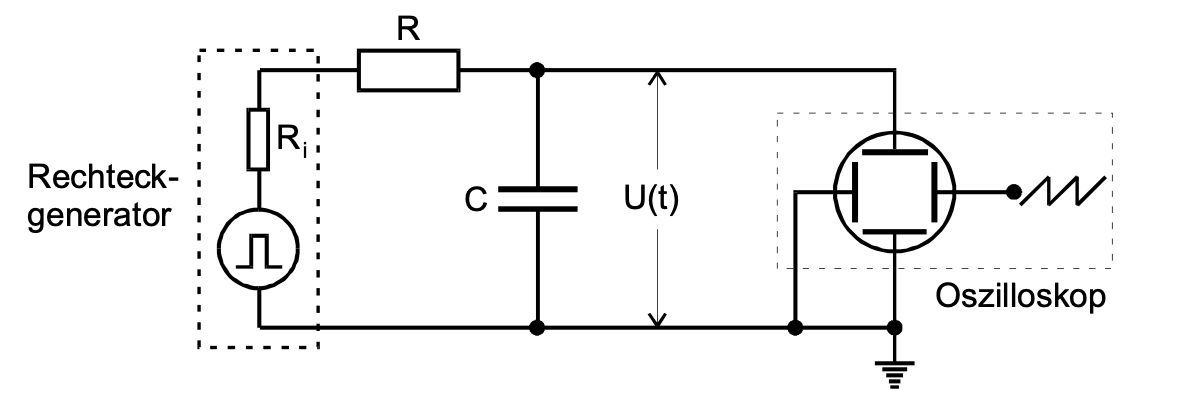
\includegraphics[height=3cm]{content/esb1.png}
    \caption{Das Ersatzschaltbild zu Teilaufgabe a)}
    \label{fig:esb1}
\end{figure}

Dazu werden Auf- und Entladevorgänge des Kondensators 
durch eine Rechteckspannung herbeigeführt und auf dem Oszilloskop die Kondensatorspannung in 
Abhängigkeit davon beobachtet. \\


Die Teilaufgabe \textbf{b)} sieht vor, dass man die Schaltung aus Abbildung~\ref{fig:esb2} die Generatorspannung in Sinusform umstellt.

\begin{figure}
    
    \centering
    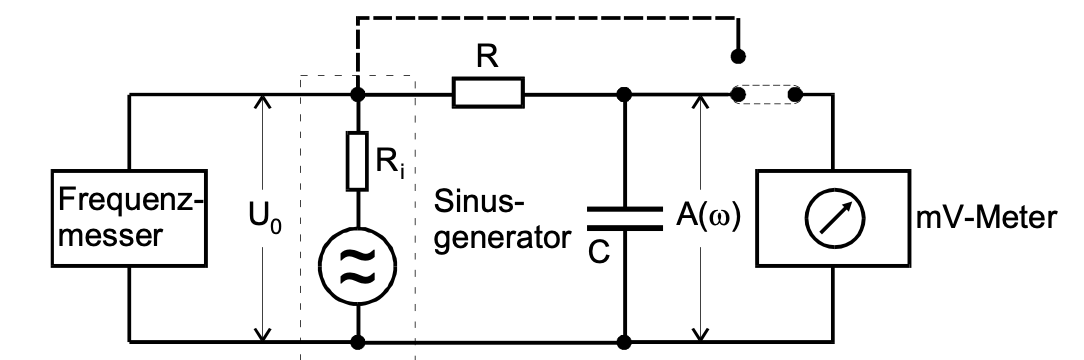
\includegraphics[height=3cm]{content/esb2.png}
    \caption{Das Ersatzschaltbild zu Aufgabe b) und c)}
    \label{fig:esb2}
\end{figure}

Gemessen werden soll hier die Amplitude $A(\omega)$ der Kondensatorspannung
 $U_C = A(\omega) \cdot \textrm{cos}(\omega t + \varphi(\omega))$ in Abhängigkeit der Frequenz
der Sinusspannung.\\

\textbf{c)} ist die Bestimmung der Phasenverschiebung zwischen Kondensator- und 
Generatorspannung in Abhängigkeit von der Frequenz der Sinusspannung. 

Es wird erneut die Schaltung aus Abbildung~\ref{fig:esb2} genutzt.

Die Amplitude der Kondensatorspannung, die zeitliche Differenz der Nulldurchgänge und die Periodendauer für \textbf{b)} und \textbf{c)} konnten in einem 
Messdurchgang vom Oszilloskop abgelesen werden werden, während dessen die Frequenz in kleinen Schritten erhöht wird. \\

In Teilaufgabe \textbf{d)} wird bewiesen, dass die vorliegende Schaltung \ref{fig:esb3} als Integrator genutzt werden kann.

\begin{figure}
    
    \centering
    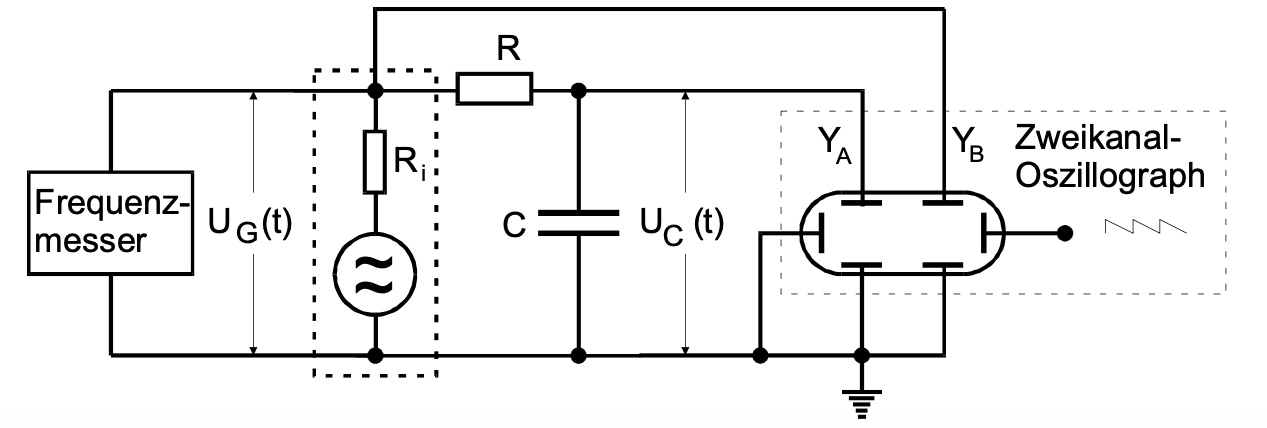
\includegraphics[height=3cm]{content/esb3.png}
    \caption{Das Ersatzschaltbild zu Teilaufgabe d)}
    \label{fig:esb3}
\end{figure}

Hierzu stellt man nacheinander eine Rechteck-, Dreieck- und Sinusspannung am Generator ein und dokumentiert 
fotographisch, wie in \ref{fig:abb9} und \ref{fig:abb10} zu sehen, die auf dem Oszilloskop angezeigte Kondensatorspannung, 
die proportional zum Integral der Generatorspannung über die Zeit sein sollte. \\




